\documentclass[aspectratio=169,12pt]{beamer}
\usepackage[utf8]{inputenc}
\usepackage{amsmath, amssymb}
\usepackage{booktabs}
\usepackage{colortbl}
\usepackage{hyperref}
\usepackage{makecell}
\usepackage{ragged2e}
\usepackage{bytefield}
\usepackage{tikz}
\usetikzlibrary{arrows.meta, positioning, shapes.geometric, calc, tikzmark, shapes.misc}
\usepackage{tcolorbox}
\usetheme{Madrid}
\title{Hardware Security Mechanisms}
\subtitle{Computer Architecture}
\author{Course 234267}
\date{}
\begin{document}
\frame{\titlepage}

% Outline
\begin{frame}{Outline}
    \tableofcontents
\end{frame}

% Additional slides to be inserted into the main presentation

% Section: Threat Model and Defense Strategy
\section{Threat Model and Defense Strategy}

\begin{frame}{Understanding Threat Models}
    \begin{columns}
        \begin{column}{0.5\textwidth}
            \textbf{What is a Threat Model?}
            \begin{itemize}
                \item Systematic analysis of:
                \begin{itemize}
                    \item What are we protecting?
                    \item Who are the attackers?
                    \item What capabilities do they have?
                    \item What are acceptable risks?
                \end{itemize}
            \end{itemize}
            
            \vspace{0.3cm}
            \textbf{Named Threat Models:}
            \begin{itemize}
                \item \textbf{Evil Maid:} Physical access when unattended
                \item \textbf{Honest but Curious:} Cloud provider with data access
                \item \textbf{Supply Chain:} Compromised hardware/firmware
            \end{itemize}
            
            \vspace{0.3cm}
            \textbf{Attacker Capabilities:}
            \begin{itemize}
                \item \textcolor{green!60!black}{User-level code execution}
                \item \textcolor{orange}{Memory corruption bugs}
                \item \textcolor{red}{Kernel vulnerabilities}
                \item \textcolor{red!80!black}{Physical access}
            \end{itemize}
        \end{column}
        \begin{column}{0.5\textwidth}
            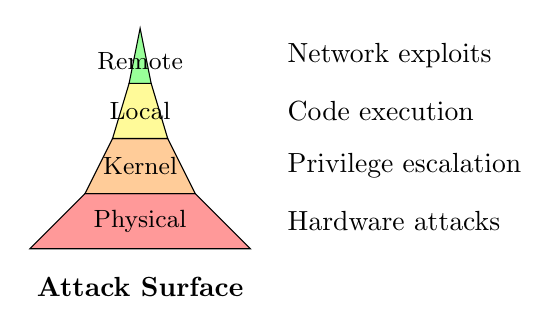
\begin{tikzpicture}[scale=0.7]
                % Threat levels pyramid
                \draw[fill=red!40] (0,0) -- (4,0) -- (3,1) -- (1,1) -- cycle;
                \node at (2,0.5) {\small Physical};
                
                \draw[fill=orange!40] (1,1) -- (3,1) -- (2.5,2) -- (1.5,2) -- cycle;
                \node at (2,1.5) {\small Kernel};
                
                \draw[fill=yellow!40] (1.5,2) -- (2.5,2) -- (2.2,3) -- (1.8,3) -- cycle;
                \node at (2,2.5) {\small Local};
                
                \draw[fill=green!40] (1.8,3) -- (2.2,3) -- (2,4) -- cycle;
                \node at (2,3.4) {\small Remote};
                
                % Labels
                \node[right] at (4.5,0.5) {Hardware attacks};
                \node[right] at (4.5,1.5) {Privilege escalation};
                \node[right] at (4.5,2.5) {Code execution};
                \node[right] at (4.5,3.5) {Network exploits};
                
                \node at (2,-0.7) {\textbf{Attack Surface}};
            \end{tikzpicture}
        \end{column}
    \end{columns}
    
    \vspace{0.5cm}
    \begin{tcolorbox}[colback=blue!10]
        \textbf{Modern CPU Security Mechanisms Target:}
        \begin{itemize}
            \item Memory corruption exploitation (buffer overflows, use-after-free)
            \item Control flow hijacking (ROP, JOP, code injection)
            \item Privilege escalation (kernel exploitation)
            \item Side-channel attacks (Spectre, Meltdown)
        \end{itemize}
    \end{tcolorbox}
\end{frame}

\begin{frame}{Defense in Depth}
    \begin{center}
        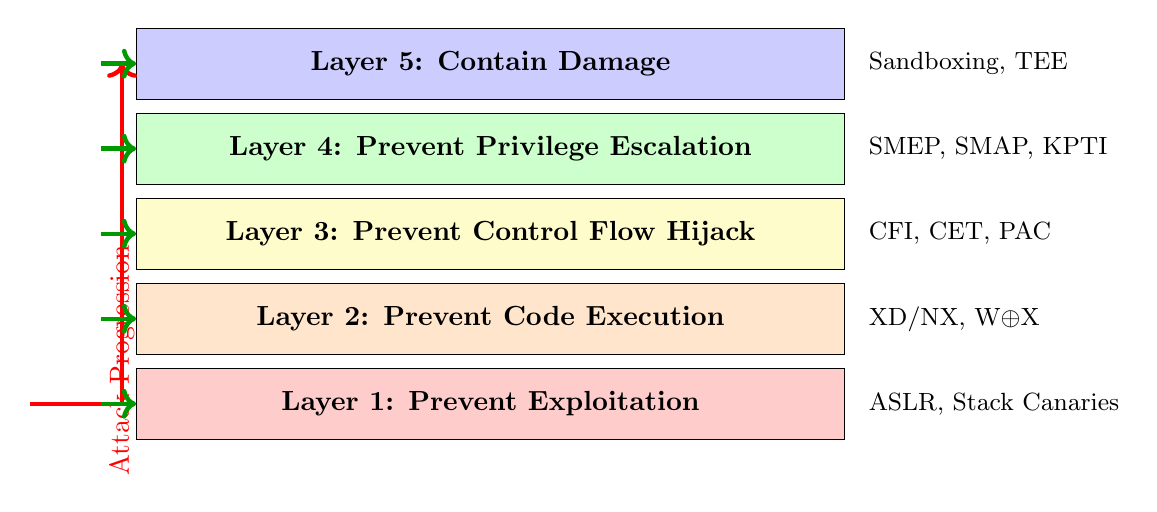
\begin{tikzpicture}[scale=0.9]
            % Castle defense layers
            \draw[fill=red!20] (0,0) rectangle (10,1);
            \node at (5,0.5) {\textbf{Layer 1: Prevent Exploitation}};
            \node[right] at (10.2,0.5) {\small ASLR, Stack Canaries};
            
            \draw[fill=orange!20] (0,1.2) rectangle (10,2.2);
            \node at (5,1.7) {\textbf{Layer 2: Prevent Code Execution}};
            \node[right] at (10.2,1.7) {\small XD/NX, W$\oplus$X};
            
            \draw[fill=yellow!20] (0,2.4) rectangle (10,3.4);
            \node at (5,2.9) {\textbf{Layer 3: Prevent Control Flow Hijack}};
            \node[right] at (10.2,2.9) {\small CFI, CET, PAC};
            
            \draw[fill=green!20] (0,3.6) rectangle (10,4.6);
            \node at (5,4.1) {\textbf{Layer 4: Prevent Privilege Escalation}};
            \node[right] at (10.2,4.1) {\small SMEP, SMAP, KPTI};
            
            \draw[fill=blue!20] (0,4.8) rectangle (10,5.8);
            \node at (5,5.3) {\textbf{Layer 5: Contain Damage}};
            \node[right] at (10.2,5.3) {\small Sandboxing, TEE};
            
            % Attack progression arrow
            \draw[->,ultra thick,red] (-1.5,0.5) -- (-0.2,0.5) -- (-0.2,5.3) node[midway,left,rotate=90] {Attack Progression};
            
            % Defense layers
            \draw[<-,ultra thick,green!60!black] (0,0.5) -- (-0.5,0.5);
            \draw[<-,ultra thick,green!60!black] (0,1.7) -- (-0.5,1.7);
            \draw[<-,ultra thick,green!60!black] (0,2.9) -- (-0.5,2.9);
            \draw[<-,ultra thick,green!60!black] (0,4.1) -- (-0.5,4.1);
            \draw[<-,ultra thick,green!60!black] (0,5.3) -- (-0.5,5.3);
        \end{tikzpicture}
    \end{center}
    
    \vspace{0.3cm}
    \begin{tcolorbox}[colback=yellow!20]
        \centering
        \textbf{Principle:} No single defense is perfect - multiple independent layers increase attack complexity exponentially
    \end{tcolorbox}
\end{frame}

% Section: ROP Protection Evolution
\section{ROP Protection Evolution}

\begin{frame}{Execute Disable (XD/NX) Bit - The First Line}
    \begin{columns}
        \begin{column}{0.5\textwidth}
            \textbf{XD/NX Bit Basics:}
            \begin{itemize}
                \item Intel: XD (eXecute Disable)
                \item AMD: NX (No eXecute)
                \item ARM: XN (eXecute Never)
                \item Page table bit 63
            \end{itemize}
            
            \vspace{0.3cm}
            \textbf{How it Works:}
            \begin{itemize}
                \item Marks memory pages non-executable
                \item CPU raises \#PF on exec attempt
                \item Enforces W$\oplus$X policy
            \end{itemize}
        \end{column}
        \begin{column}{0.5\textwidth}
            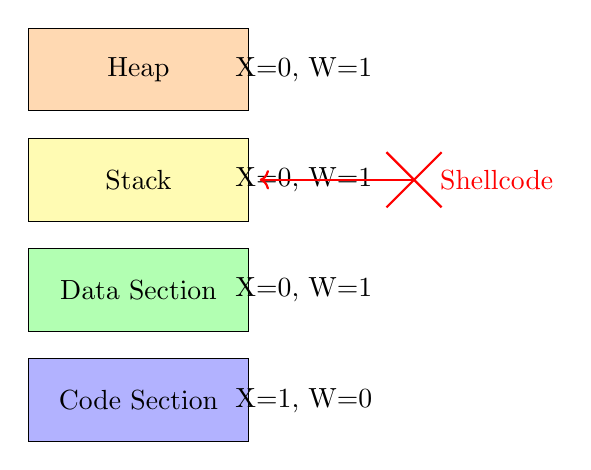
\begin{tikzpicture}[scale=0.7]
                % Memory layout
                \draw[fill=blue!30] (0,0) rectangle (4,1.5);
                \node at (2,0.75) {Code Section};
                \node at (5,0.75) {X=1, W=0};
                
                \draw[fill=green!30] (0,2) rectangle (4,3.5);
                \node at (2,2.75) {Data Section};
                \node at (5,2.75) {X=0, W=1};
                
                \draw[fill=yellow!30] (0,4) rectangle (4,5.5);
                \node at (2,4.75) {Stack};
                \node at (5,4.75) {X=0, W=1};
                
                \draw[fill=orange!30] (0,6) rectangle (4,7.5);
                \node at (2,6.75) {Heap};
                \node at (5,6.75) {X=0, W=1};
                
                % Attack blocked
                \draw[->,thick,red] (7,4.75) -- (4.2,4.75);
                \node[red] at (8.5,4.75) {Shellcode};
                \draw[red,thick] (6.5,4.25) -- (7.5,5.25);
                \draw[red,thick] (6.5,5.25) -- (7.5,4.25);
            \end{tikzpicture}
            
            \vspace{0.3cm}
            \textbf{What XD Prevents:}
            \begin{itemize}
                \item Classic buffer overflow + shellcode
                \item Direct code injection attacks
            \end{itemize}
        \end{column}
    \end{columns}
\end{frame}

\begin{frame}[fragile]{Why XD/NX is Not Enough - Enter ROP}
    \begin{columns}
        \begin{column}{0.5\textwidth}
            \textbf{The Problem:}
            \begin{itemize}
                \item Attackers don't need new code!
                \item Existing code has everything needed
                \item Chain existing code snippets
            \end{itemize}
            
            \vspace{0.3cm}
            \textbf{Return-Oriented Programming:}
            \begin{itemize}
                \item Uses "gadgets" ending in RET
                \item Gadget = useful instruction(s) + RET
                \item Chain gadgets via stack control
                \item Turing complete!
            \end{itemize}
        \end{column}
        \begin{column}{0.5\textwidth}
            \begin{tcolorbox}[colback=gray!10]
                \small
                \textbf{ROP Attack Example:}
                \begin{verbatim}
; Gadget 1: pop rdi; ret
; Gadget 2: pop rsi; ret  
; Gadget 3: mov rax, 59; ret
; Gadget 4: syscall

Stack Layout:
[addr_gadget1]
["/bin/sh"]
[addr_gadget2]
[0]
[addr_gadget3]
[addr_gadget4]
                \end{verbatim}
            \end{tcolorbox}
            
            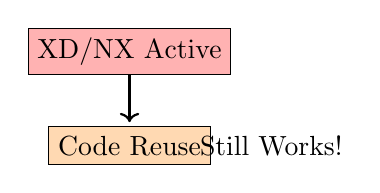
\begin{tikzpicture}[scale=0.6]
                \node[draw,fill=red!30] at (0,0) {XD/NX Active};
                \draw[->,thick] (0,-0.5) -- (0,-1.5);
                \node[draw,fill=orange!30] at (0,-2) {Code Reuse};
                \node at (3,-2) {Still Works!};
            \end{tikzpicture}
        \end{column}
    \end{columns}
\end{frame}

\begin{frame}{ROP Attack Visualization}
    \begin{center}
        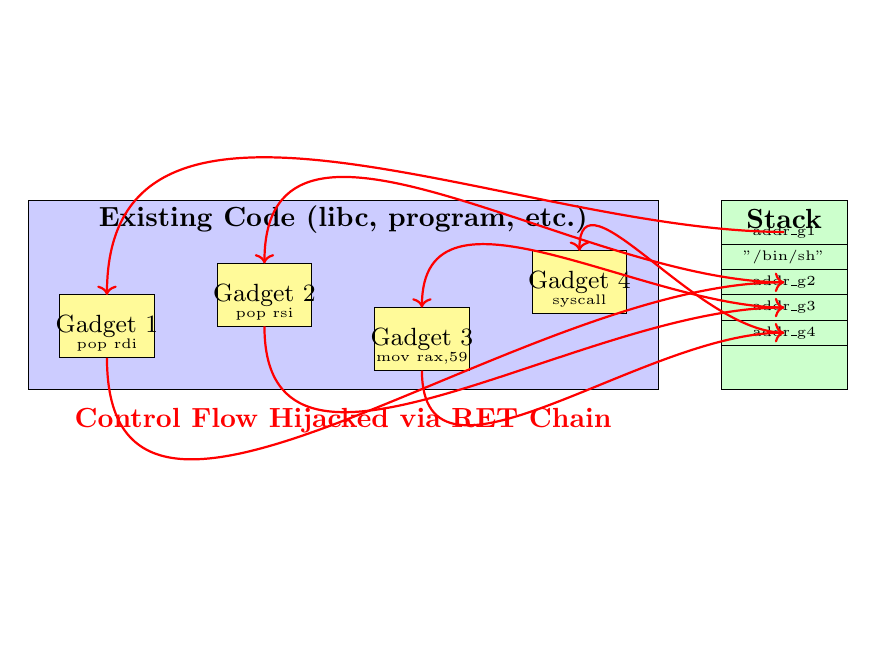
\begin{tikzpicture}[scale=0.8]
            % Code section
            \draw[fill=blue!20] (0,0) rectangle (10,3);
            \node at (5,2.7) {\textbf{Existing Code (libc, program, etc.)}};
            
            % Gadgets
            \draw[fill=yellow!40] (0.5,0.5) rectangle (2,1.5);
            \node at (1.25,1) {\small Gadget 1};
            \node at (1.25,0.7) {\tiny pop rdi};
            
            \draw[fill=yellow!40] (3,1) rectangle (4.5,2);
            \node at (3.75,1.5) {\small Gadget 2};
            \node at (3.75,1.2) {\tiny pop rsi};
            
            \draw[fill=yellow!40] (5.5,0.3) rectangle (7,1.3);
            \node at (6.25,0.8) {\small Gadget 3};
            \node at (6.25,0.5) {\tiny mov rax,59};
            
            \draw[fill=yellow!40] (8,1.2) rectangle (9.5,2.2);
            \node at (8.75,1.7) {\small Gadget 4};
            \node at (8.75,1.4) {\tiny syscall};
            
            % Stack
            \draw[fill=green!20] (11,0) rectangle (13,3);
            \node at (12,2.7) {\textbf{Stack}};
            
            % ROP chain on stack
            \draw (11,2.3) -- (13,2.3);
            \node at (12,2.5) {\tiny addr\_g1};
            \draw (11,1.9) -- (13,1.9);
            \node at (12,2.1) {\tiny "/bin/sh"};
            \draw (11,1.5) -- (13,1.5);
            \node at (12,1.7) {\tiny addr\_g2};
            \draw (11,1.1) -- (13,1.1);
            \node at (12,1.3) {\tiny addr\_g3};
            \draw (11,0.7) -- (13,0.7);
            \node at (12,0.9) {\tiny addr\_g4};
            
            % Execution flow
            \draw[->,thick,red] (12,2.5) to[out=180,in=90] (1.25,1.5);
            \draw[->,thick,red] (1.25,0.5) to[out=-90,in=180] (12,1.7);
            \draw[->,thick,red] (12,1.7) to[out=180,in=90] (3.75,2);
            \draw[->,thick,red] (3.75,1) to[out=-90,in=180] (12,1.3);
            \draw[->,thick,red] (12,1.3) to[out=180,in=90] (6.25,1.3);
            \draw[->,thick,red] (6.25,0.3) to[out=-90,in=180] (12,0.9);
            \draw[->,thick,red] (12,0.9) to[out=180,in=90] (8.75,2.2);
            
            \node[red] at (5,-0.5) {\textbf{Control Flow Hijacked via RET Chain}};
        \end{tikzpicture}
    \end{center}
    
    \begin{tcolorbox}[colback=red!10]
        \textbf{Key Insight:} ROP bypasses XD/NX by reusing existing executable code - no code injection needed!
    \end{tcolorbox}
\end{frame}

% Section: SMEP and SMAP
\section{Kernel Protection: SMEP and SMAP}

\begin{frame}{SMEP - Supervisor Mode Execution Prevention}
    \begin{columns}
        \begin{column}{0.5\textwidth}
            \textbf{The Problem:}
            \begin{itemize}
                \item Kernel exploits redirect to user code
                \item User controls memory at known addresses
                \item ret2user attacks bypass KASLR
            \end{itemize}
            
            \vspace{0.3cm}
            \textbf{SMEP Solution:}
            \begin{itemize}
                \item CR4.SMEP bit (bit 20)
                \item Prevents kernel executing user pages
                \item \#PF if CPL=0 tries to execute U=1 page
                \item Intel: Ivy Bridge (2012)
            \end{itemize}
        \end{column}
        \begin{column}{0.5\textwidth}
            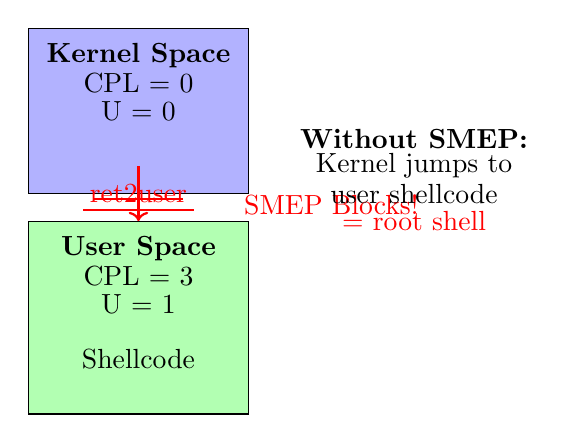
\begin{tikzpicture}[scale=0.7]
                % Memory layout
                \draw[fill=blue!30] (0,4) rectangle (4,7);
                \node at (2,6.5) {\textbf{Kernel Space}};
                \node at (2,6) {CPL = 0};
                \node at (2,5.5) {U = 0};
                
                \draw[fill=green!30] (0,0) rectangle (4,3.5);
                \node at (2,3) {\textbf{User Space}};
                \node at (2,2.5) {CPL = 3};
                \node at (2,2) {U = 1};
                \node at (2,1) {Shellcode};
                
                % Attack attempt
                \draw[->,thick,red] (2,4.5) -- (2,3.5);
                \node[red] at (2,4) {ret2user};
                
                % SMEP blocks
                \draw[thick,red] (1,3.7) -- (3,3.7);
                \draw[thick,red] (1.2,3.9) -- (2.8,3.9);
                \node[red] at (5.5,3.8) {SMEP Blocks!};
                
                % Without SMEP
                \node at (7,5) {\textbf{Without SMEP:}};
                \node at (7,4.5) {Kernel jumps to};
                \node at (7,4) {user shellcode};
                \node[red] at (7,3.5) {= root shell};
            \end{tikzpicture}
        \end{column}
    \end{columns}
    
    \vspace{0.3cm}
    \begin{tcolorbox}[colback=yellow!20]
        \textbf{Bypass Methods:} ROP in kernel code, physmap spraying, page table manipulation
    \end{tcolorbox}
\end{frame}

\begin{frame}[fragile]{SMAP - Supervisor Mode Access Prevention}
    \begin{columns}
        \begin{column}{0.5\textwidth}
            \textbf{The Problem After SMEP:}
            \begin{itemize}
                \item Can't execute user pages
                \item But can still READ/WRITE them!
                \item Kernel ROP can use user data
                \item Arbitrary write to user buffers
            \end{itemize}
            
            \vspace{0.3cm}
            \textbf{SMAP Solution:}
            \begin{itemize}
                \item CR4.SMAP bit (bit 21)
                \item Blocks kernel access to user pages
                \item STAC/CLAC instructions for legitimate access
                \item Intel: Broadwell (2014)
            \end{itemize}
        \end{column}
        \begin{column}{0.5\textwidth}
            \begin{tcolorbox}[colback=gray!10]
                \small
                \textbf{Kernel Code Pattern:}
                \begin{verbatim}
copy_from_user:
    STAC        ; Enable access
    mov (%rdi), %rax
    CLAC        ; Disable access
    ret
    
; Vulnerability example:
some_ioctl:
    ; Missing STAC/CLAC!
    mov %rsi, (%rdi)  ; Oops!
                \end{verbatim}
            \end{tcolorbox}
            
            \textbf{EFLAGS.AC bit:}
            \begin{itemize}
                \item AC=0: SMAP active (default)
                \item AC=1: Temporary user access
                \item Only changeable in Ring 0
            \end{itemize}
        \end{column}
    \end{columns}
\end{frame}

\begin{frame}{SMEP + SMAP Combined Protection}
    \begin{center}
        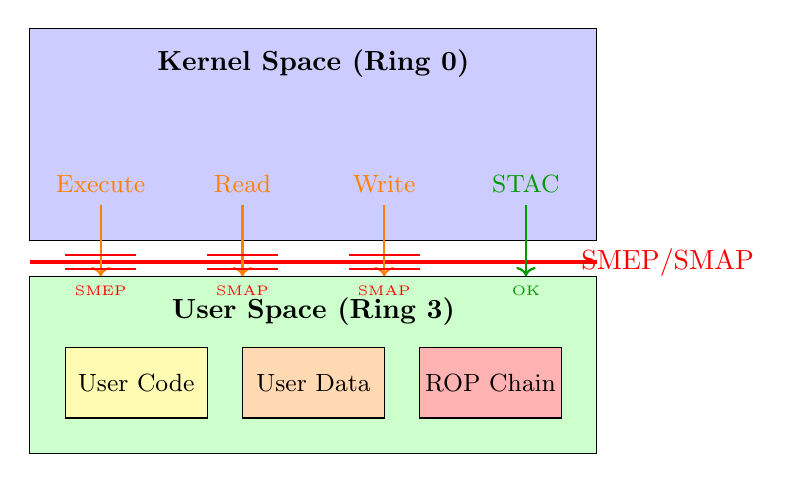
\begin{tikzpicture}[scale=0.9]
            % Kernel space
            \draw[fill=blue!20] (0,3) rectangle (8,6);
            \node at (4,5.5) {\textbf{Kernel Space (Ring 0)}};
            
            % User space
            \draw[fill=green!20] (0,0) rectangle (8,2.5);
            \node at (4,2) {\textbf{User Space (Ring 3)}};
            
            % Protection barriers
            \draw[ultra thick, red] (0,2.7) -- (8,2.7);
            \node[red] at (9,2.7) {SMEP/SMAP};
            
            % Attack scenarios
            % 1. Code execution attempt
            \draw[->,thick,orange] (1,3.5) -- (1,2.5);
            \node[orange] at (1,3.8) {\small Execute};
            \draw[thick,red] (0.5,2.6) -- (1.5,2.6);
            \draw[thick,red] (0.5,2.8) -- (1.5,2.8);
            \node[red] at (1,2.3) {\tiny SMEP};
            
            % 2. Data read attempt
            \draw[->,thick,orange] (3,3.5) -- (3,2.5);
            \node[orange] at (3,3.8) {\small Read};
            \draw[thick,red] (2.5,2.6) -- (3.5,2.6);
            \draw[thick,red] (2.5,2.8) -- (3.5,2.8);
            \node[red] at (3,2.3) {\tiny SMAP};
            
            % 3. Data write attempt
            \draw[->,thick,orange] (5,3.5) -- (5,2.5);
            \node[orange] at (5,3.8) {\small Write};
            \draw[thick,red] (4.5,2.6) -- (5.5,2.6);
            \draw[thick,red] (4.5,2.8) -- (5.5,2.8);
            \node[red] at (5,2.3) {\tiny SMAP};
            
            % 4. Legitimate access
            \draw[->,thick,green!60!black] (7,3.5) -- (7,2.5);
            \node[green!60!black] at (7,3.8) {\small STAC};
            \node[green!60!black] at (7,2.3) {\tiny OK};
            
            % User data/code
            \draw[fill=yellow!30] (0.5,0.5) rectangle (2.5,1.5);
            \node at (1.5,1) {\small User Code};
            
            \draw[fill=orange!30] (3,0.5) rectangle (5,1.5);
            \node at (4,1) {\small User Data};
            
            \draw[fill=red!30] (5.5,0.5) rectangle (7.5,1.5);
            \node at (6.5,1) {\small ROP Chain};
        \end{tikzpicture}
    \end{center}
    
    \vspace{0.3cm}
    \begin{columns}
        \begin{column}{0.5\textwidth}
            \textbf{Protection Matrix:}
            \begin{tabular}{|l|c|c|}
                \hline
                From Kernel & Execute & Access \\
                \hline
                No Protection & \checkmark & \checkmark \\
                SMEP only & $\times$ & \checkmark \\
                SMAP only & \checkmark & $\times$ \\
                SMEP+SMAP & $\times$ & $\times$* \\
                \hline
            \end{tabular}
            
            \small *Except with STAC/CLAC
        \end{column}
        \begin{column}{0.5\textwidth}
            \textbf{Remaining Attack Surface:}
            \begin{itemize}
                \item Kernel ROP/JOP only
                \item Kernel heap/stack spraying
                \item Race conditions in STAC/CLAC windows
                \item Hardware vulnerabilities (Spectre/Meltdown)
            \end{itemize}
        \end{column}
    \end{columns}
\end{frame}

\begin{frame}{Modern ROP Mitigations Summary}
    \begin{center}
        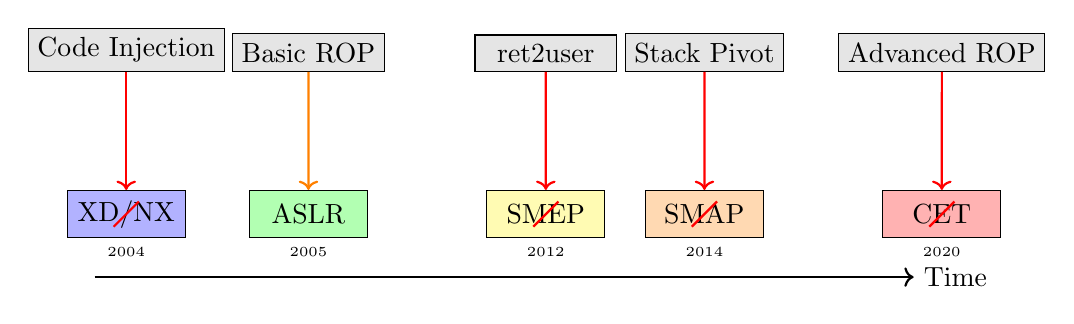
\begin{tikzpicture}[scale=0.8,
            defense/.style={draw,minimum width=1.5cm,minimum height=0.6cm},
            attack/.style={draw,fill=gray!20,minimum width=1.8cm}]
            
            % Timeline arrow
            \draw[thick,->] (-0.5,-1) -- (12.5,-1) node[right] {Time};
            
            % Defense nodes with relative positioning
            \node[defense,fill=blue!30] (nx) at (0,0) {XD/NX};
            \node[below] at (nx.south) {\tiny 2004};
            
            \node[defense,fill=green!30,right=0.8cm of nx] (aslr) {ASLR};
            \node[below] at (aslr.south) {\tiny 2005};
            
            \node[defense,fill=yellow!30,right=1.5cm of aslr] (smep) {SMEP};
            \node[below] at (smep.south) {\tiny 2012};
            
            \node[defense,fill=orange!30,right=0.5cm of smep] (smap) {SMAP};
            \node[below] at (smap.south) {\tiny 2014};
            
            \node[defense,fill=red!30,right=1.5cm of smap] (cet) {CET};
            \node[below] at (cet.south) {\tiny 2020};
            
            % Attack techniques above defenses
            \node[attack,above=1.5cm of nx] (inject) {Code Injection};
            \draw[->,thick,red] (inject) -- (nx);
            \draw[thick,red] ([shift={(-0.2,-0.2)}]nx.center) -- ([shift={(0.2,0.2)}]nx.center);
            
            \node[attack,above=1.5cm of aslr] (rop) {Basic ROP};
            \draw[->,thick,orange] (rop) -- (aslr);
            
            \node[attack,above=1.5cm of smep] (ret2user) {ret2user};
            \draw[->,thick,red] (ret2user) -- (smep);
            \draw[thick,red] ([shift={(-0.2,-0.2)}]smep.center) -- ([shift={(0.2,0.2)}]smep.center);
            
            \node[attack,above=1.5cm of smap] (pivot) {Stack Pivot};
            \draw[->,thick,red] (pivot) -- (smap);
            \draw[thick,red] ([shift={(-0.2,-0.2)}]smap.center) -- ([shift={(0.2,0.2)}]smap.center);
            
            \node[attack,above=1.5cm of cet] (advanced) {Advanced ROP};
            \draw[->,thick,red] (advanced) -- (cet);
            \draw[thick,red] ([shift={(-0.2,-0.2)}]cet.center) -- ([shift={(0.2,0.2)}]cet.center);
        \end{tikzpicture}
    \end{center}
    
    \vspace{0.5cm}
    \begin{columns}
        \begin{column}{0.33\textwidth}
            \textbf{User Space:}
            \begin{itemize}
                \item XD/NX bit
                \item ASLR
                \item Stack Canaries
                \item CFI/CET
                \item Shadow Stack
            \end{itemize}
        \end{column}
        \begin{column}{0.33\textwidth}
            \textbf{Kernel Space:}
            \begin{itemize}
                \item SMEP (HW)
                \item SMAP (HW)
                \item KASLR (SW)
                \item KPTI* (SW)
                \item FineIBT (HW+SW)
            \end{itemize}
        \end{column}
        \begin{column}{0.33\textwidth}
            \textbf{Hardware:}
            \begin{itemize}
                \item Intel CET
                \item ARM PAC/BTI
                \item ARM MTE
                \item Control-flow integrity
            \end{itemize}
        \end{column}
    \end{columns}
    
    \vspace{0.2cm}
    \small *KPTI: Kernel Page Table Isolation - software mitigation for Meltdown
\end{frame}

\begin{frame}{Performance Impact of Security Features}
    \begin{center}
        \begin{tabular}{|l|c|c|l|}
            \hline
            \textbf{Feature} & \textbf{Type} & \textbf{Impact} & \textbf{Overhead} \\
            \hline
            \hline
            XD/NX Bit & HW & \cellcolor{green!30}Low & Page table bit check \\
            \hline
            SMEP & HW & \cellcolor{green!30}Low & Permission check \\
            \hline
            SMAP & HW & \cellcolor{green!30}Low & AC flag check \\
            \hline
            Stack Canaries & SW & \cellcolor{green!30}Low & Function epilogue check \\
            \hline
            ASLR & SW & \cellcolor{green!30}Low & One-time randomization \\
            \hline
            CET (Shadow Stack) & HW & \cellcolor{yellow!30}Medium & Parallel stack ops \\
            \hline
            PAC (ARM) & HW & \cellcolor{yellow!30}Medium & Crypto ops per call \\
            \hline
            BTI (ARM) & HW & \cellcolor{yellow!30}Medium & Branch checks \\
            \hline
            KASLR & SW & \cellcolor{yellow!30}Medium & Kernel relocation \\
            \hline
            KPTI* & SW & \cellcolor{orange!30}High & Page table switches \\
            \hline
            Full CFI** & SW & \cellcolor{orange!30}High & Type checks everywhere \\
            \hline
            FineIBT & HW+SW & \cellcolor{yellow!30}Medium & Hash + branch checks \\
            \hline
        \end{tabular}
    \end{center}
    
    \vspace{0.3cm}
    \begin{columns}
        \begin{column}{0.5\textwidth}
            \small
            *Software mitigation for Meltdown\\
            **Software-only implementation
        \end{column}
        \begin{column}{0.5\textwidth}
            \begin{tcolorbox}[colback=yellow!10]
                \small
                \textbf{Impact Categories:}
                \begin{itemize}
                    \item \textcolor{green!70!black}{Low}: $<$5\%
                    \item \textcolor{yellow!70!black}{Medium}: 5-15\%
                    \item \textcolor{orange!70!black}{High}: $>$15\%
                \end{itemize}
            \end{tcolorbox}
        \end{column}
    \end{columns}
\end{frame}

% Section 1: Memory Protection
\section{Memory Protection Mechanisms}

\begin{frame}{Pointer Tagging}
    \begin{columns}
        \begin{column}{0.5\textwidth}
            \textbf{Concept:}
            \begin{itemize}
                \item Uses unused bits in 64-bit pointers
                \item Tags store metadata (type, color, version)
                \item Enables memory safety checks
            \end{itemize}
            
            \vspace{0.5cm}
            \textbf{Benefits:}
            \begin{itemize}
                \item Detect use-after-free
                \item Prevent type confusion
                \item Low overhead ($<$5\%)
            \end{itemize}
        \end{column}
        \begin{column}{0.5\textwidth}
            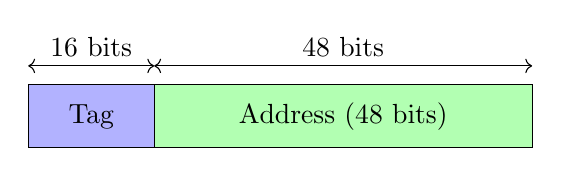
\begin{tikzpicture}[scale=0.8]
                \draw (0,0) rectangle (8,1);
                \draw[fill=blue!30] (0,0) rectangle (2,1);
                \draw[fill=green!30] (2,0) rectangle (8,1);
                \node at (1,0.5) {Tag};
                \node at (5,0.5) {Address (48 bits)};
                \draw[<->] (0,1.3) -- (2,1.3) node[midway,above] {16 bits};
                \draw[<->] (2,1.3) -- (8,1.3) node[midway,above] {48 bits};
            \end{tikzpicture}
            
            \vspace{0.5cm}
            \textbf{Example: ARM MTE}
            \begin{itemize}
                \item 4-bit tags in bits [59:56]
                \item Hardware tag checking
                \item Synchronous/async exceptions
            \end{itemize}
        \end{column}
    \end{columns}
\end{frame}

\begin{frame}[fragile]{Pointer Authentication (PAC)}
    \begin{columns}
        \begin{column}{0.5\textwidth}
            \textbf{ARM PAC Architecture:}
            \begin{itemize}
                \item Cryptographic signature in pointer
                \item Uses QARMA block cipher
                \item 5 128-bit keys (IA, IB, DA, DB, GA)
            \end{itemize}
            
            \vspace{0.3cm}
            \textbf{Operations:}
            \begin{itemize}
                \item \texttt{PACIA}: Sign instruction pointer
                \item \texttt{AUTIA}: Authenticate pointer
                \item \texttt{PACDA}: Sign data pointer
            \end{itemize}
        \end{column}
        \begin{column}{0.5\textwidth}
            \begin{tcolorbox}[colback=gray!10]
                \small
                \textbf{Function Prologue:}
                \begin{verbatim}
PACIASP    ; Sign LR with SP
STP x29,x30,[sp,#-16]!
                \end{verbatim}
                
                \textbf{Function Epilogue:}
                \begin{verbatim}
LDP x29,x30,[sp],#16
AUTIASP    ; Verify LR
RET        ; Return if valid
                \end{verbatim}
            \end{tcolorbox}
            
            \vspace{0.2cm}
            \textbf{Key Terms:}
            \begin{itemize}
                \item \textbf{LR (x30):} Link Register - stores return address
                \item \textbf{SP:} Stack Pointer - used as context
                \item \textbf{x29:} Frame Pointer
            \end{itemize}
            
            \textbf{Security:} Prevents ROP/JOP attacks
        \end{column}
    \end{columns}
\end{frame}

% Section 2: Control Flow Integrity
\section{Control Flow Integrity}

\begin{frame}{Control Flow Integrity (CFI) - Overview}
    \begin{columns}
        \begin{column}{0.5\textwidth}
            \textbf{Core Concept:}
            \begin{itemize}
                \item Enforce legitimate control flow transfers
                \item Prevent code-reuse attacks (ROP/JOP/COP)
                \item Hardware + software enforcement
            \end{itemize}
            
            \vspace{0.3cm}
            \textbf{Two Protection Categories:}
            
            \colorbox{green!20}{\textbf{Forward-Edge CFI:}}
            \begin{itemize}
                \item Indirect calls (call rax)
                \item Indirect jumps (jmp rbx)
                \item Virtual function calls
            \end{itemize}
            
            \colorbox{blue!20}{\textbf{Backward-Edge CFI:}}
            \begin{itemize}
                \item Function returns (ret)
                \item Return address integrity
            \end{itemize}
        \end{column}
        \begin{column}{0.5\textwidth}
            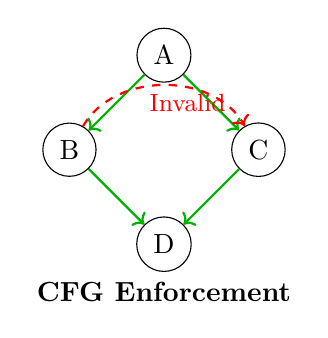
\begin{tikzpicture}[scale=0.6]
                % Control flow graph
                \node[draw,circle] (A) at (2,4) {A};
                \node[draw,circle] (B) at (0,2) {B};
                \node[draw,circle] (C) at (4,2) {C};
                \node[draw,circle] (D) at (2,0) {D};
                
                % Valid edges (green)
                \draw[->,thick,green!70!black] (A) -- (B);
                \draw[->,thick,green!70!black] (A) -- (C);
                \draw[->,thick,green!70!black] (B) -- (D);
                \draw[->,thick,green!70!black] (C) -- (D);
                
                % Invalid edge (red, dashed)
                \draw[->,thick,red,dashed] (B) to[bend left=60] (C);
                \node[red] at (2.5,3) {\small Invalid};
                
                \node at (2,-1) {\textbf{CFG Enforcement}};
            \end{tikzpicture}
            
            \vspace{0.3cm}
            \begin{tcolorbox}[colback=yellow!10]
                \small
                \textbf{Attack Example:}
                Attacker overwrites function pointer to jump from B→C, violating intended control flow
            \end{tcolorbox}
        \end{column}
    \end{columns}
\end{frame}

\begin{frame}[fragile]{Forward-Edge CFI Mechanisms}
    \begin{columns}
        \begin{column}{0.5\textwidth}
            \textbf{Intel CET-IBT (Indirect Branch Tracking):}
            \begin{itemize}
                \item \texttt{ENDBRANCH} instruction marks valid targets
                \item CPU tracks indirect branch state
                \item Fault if target lacks \texttt{ENDBRANCH}
            \end{itemize}
            
            \vspace{0.3cm}
            \textbf{ARM BTI (Branch Target Identification):}
            \begin{itemize}
                \item \texttt{BTI} instructions mark valid targets
                \item Variants match branch types:
                \begin{itemize}
                    \item \texttt{BTI c}: Call target (BLR)
                    \item \texttt{BTI j}: Jump target (BR)
                    \item \texttt{BTI jc}: Both call \& jump
                \end{itemize}
                \item CPU faults on mismatch
            \end{itemize}
            
            \vspace{0.3cm}
            \textbf{Software CFI (LLVM):}
            \begin{itemize}
                \item Type-based: Check function signatures
                \item Fine-grained: Unique IDs per callsite
                \item Cross-DSO support
            \end{itemize}
        \end{column}
        \begin{column}{0.5\textwidth}
            \begin{tcolorbox}[colback=gray!10]
                \small
                \textbf{Example: Intel CET-IBT}
                \begin{verbatim}
valid_target:
    endbranch    ; Mark as valid
    push rbp
    mov rbp, rsp
    ; Function body
    
invalid_target:  ; No endbranch
    push rbp     ; CPU fault here!
    mov rbp, rsp
                \end{verbatim}
            \end{tcolorbox}
            
            \textbf{Protection Granularity:}
            \begin{itemize}
                \item \textbf{Coarse:} Any valid function
                \item \textbf{Fine:} Type-compatible functions
                \item \textbf{Ultra-fine:} Exact callsite matching
            \end{itemize}
        \end{column}
    \end{columns}
\end{frame}

\begin{frame}[fragile]{ARM BTI Explained}
    \begin{columns}
        \begin{column}{0.5\textwidth}
            \textbf{BTI Instruction Variants:}
            \begin{itemize}
                \item \textbf{BTI c}: Target of calls (BLR/BLRA)
                \item \textbf{BTI j}: Target of jumps (BR/BRA)
                \item \textbf{BTI jc}: Target of both
                \item \textbf{BTI}: Same as BTI jc (alias)
            \end{itemize}
            
            \vspace{0.3cm}
            \textbf{How It Works:}
            \begin{enumerate}
                \item Indirect branch sets PSTATE.BTYPE
                \item Target instruction checked
                \item Must be correct BTI variant
                \item Otherwise: exception generated
            \end{enumerate}
            
            \vspace{0.3cm}
            \textbf{Use Cases:}
            \begin{itemize}
                \item Function entry points: BTI c
                \item Switch jump tables: BTI j
                \item PLT stubs: BTI jc
            \end{itemize}
        \end{column}
        \begin{column}{0.5\textwidth}
            \begin{tcolorbox}[colback=gray!10]
                \small
                \textbf{BTI Usage Example:}
                \begin{verbatim}
; Function called via pointer
func_ptr:
    BTI c      ; Mark as call target
    stp x29, x30, [sp, #-16]!
    ; Function body
    ldp x29, x30, [sp], #16
    ret

; Jump table target
case_handler:
    BTI j      ; Mark as jump target
    ; Handle case
    ret

; PLT stub (can be called or jumped to)
plt_stub:
    BTI jc     ; Both call and jump
    adrp x16, GOT_ENTRY
    ldr x17, [x16, #:lo12:GOT_ENTRY]
    br x17
                \end{verbatim}
            \end{tcolorbox}
        \end{column}
    \end{columns}
\end{frame}

\begin{frame}{Backward-Edge CFI Mechanisms}
    \begin{columns}
        \begin{column}{0.5\textwidth}
            \textbf{Stack Canaries (Software, 1998):}
            \begin{itemize}
                \item Random value before return address
                \item Check before function return
                \item Limited protection (info leak bypass)
                \item Compiler support (GCC -fstack-protector)
            \end{itemize}
            
            \vspace{0.3cm}
            \textbf{Pointer Authentication (PAC, 2018):}
            \begin{itemize}
                \item Cryptographic signing of return address
                \item ARM-specific hardware feature
                \item Key-based authentication
                \item Related to canaries but much stronger
            \end{itemize}
            
            \vspace{0.3cm}
            \textbf{Shadow Stack (Hardware, 2020):}
            \begin{itemize}
                \item Parallel stack for return addresses
                \item Intel CET-SS, ARM GCS
                \item Automatic push/pop on CALL/RET
            \end{itemize}
        \end{column}
        \begin{column}{0.5\textwidth}
            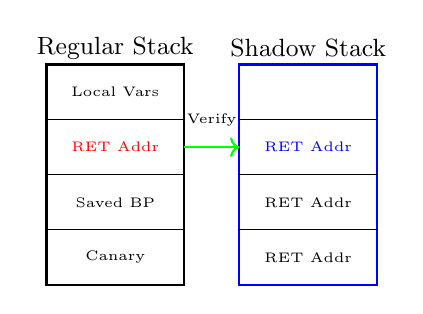
\begin{tikzpicture}[scale=0.7]
                % Regular stack
                \draw[thick] (0,0) rectangle (2.5,4);
                \node at (1.25,4.3) {\small Regular Stack};
                \draw (0,3) -- (2.5,3);
                \node at (1.25,3.5) {\tiny Local Vars};
                \draw (0,2) -- (2.5,2);
                \node[red] at (1.25,2.5) {\tiny RET Addr};
                \draw (0,1) -- (2.5,1);
                \node at (1.25,1.5) {\tiny Saved BP};
                \node at (1.25,0.5) {\tiny Canary};
                
                % Shadow stack
                \draw[thick,blue] (3.5,0) rectangle (6,4);
                \node at (4.75,4.3) {\small Shadow Stack};
                \draw (3.5,3) -- (6,3);
                \draw (3.5,2) -- (6,2);
                \node[blue] at (4.75,2.5) {\tiny RET Addr};
                \draw (3.5,1) -- (6,1);
                \node at (4.75,1.5) {\tiny RET Addr};
                \node at (4.75,0.5) {\tiny RET Addr};
                
                % Verification arrow
                \draw[->,thick,green] (2.5,2.5) -- (3.5,2.5);
                \node at (3,3) {\tiny Verify};
            \end{tikzpicture}
            
            \vspace{0.3cm}
            \begin{tcolorbox}[colback=orange!10]
                \textbf{Comparison:}
                \begin{itemize}
                    \item Shadow Stack: Strongest, hardware
                    \item PAC: Strong, ARM-only
                    \item Canaries: Weakest, portable
                \end{itemize}
            \end{tcolorbox}
        \end{column}
    \end{columns}
\end{frame}

\begin{frame}[fragile]{The Type Confusion Problem}
    \begin{columns}
        \begin{column}{0.5\textwidth}
            \textbf{What is Type Confusion?}
            \begin{itemize}
                \item Object interpreted as wrong type
                \item Common in C++ with inheritance
                \item Enables control flow hijacking
                \item Bypass basic CFI checks
            \end{itemize}
            
            \vspace{0.3cm}
            \textbf{Attack Scenario:}
            \begin{itemize}
                \item Attacker controls object allocation
                \item Forces type confusion via UAF/overflow
                \item Calls virtual function on wrong type
                \item Jumps to attacker-controlled vtable
            \end{itemize}
            
            \vspace{0.3cm}
            \textbf{Why Basic CFI Fails:}
            \begin{itemize}
                \item All virtual calls are "valid" targets
                \item Cannot distinguish object types
                \item Need type-aware CFI (FineIBT)
            \end{itemize}
        \end{column}
        \begin{column}{0.5\textwidth}
            \begin{tcolorbox}[colback=gray!10]
                \small
                \textbf{Type Confusion Example:}
                \begin{verbatim}
class Animal {
  virtual void speak() = 0;
};

class Dog : public Animal {
  void speak() { bark(); }
};

class Cat : public Animal {
  void speak() { meow(); }
  void admin() { system("/bin/sh"); }
};

// Vulnerability:
Animal* ptr = getDog();
// Type confusion happens here!
Cat* evil = (Cat*)ptr;
evil->admin(); // Calls wrong vtable!
                \end{verbatim}
            \end{tcolorbox}
            
            \begin{tcolorbox}[colback=red!10]
                \small
                \textbf{Impact:} Attacker calls admin() on Dog object, leading to arbitrary code execution
            \end{tcolorbox}
        \end{column}
    \end{columns}
\end{frame}

\begin{frame}[fragile]{FineIBT - Advanced Forward-Edge CFI}
    \begin{columns}
        \begin{column}{0.5\textwidth}
            \textbf{Linux Kernel Implementation:}
            \begin{itemize}
                \item Combines Intel CET-IBT with kCFI
                \item Function type hash validation
                \item Per-function-signature protection
            \end{itemize}
            
            \vspace{0.3cm}
            \textbf{How it Works:}
            \begin{enumerate}
                \item Compiler generates type hash
                \item Hash checked at indirect call site
                \item ENDBRANCH validates branch target
                \item Mismatch triggers exception
            \end{enumerate}
            
            \vspace{0.3cm}
            \textbf{Benefits over Basic IBT:}
            \begin{itemize}
                \item Type safety enforcement
                \item Prevents type confusion attacks
                \item Minimal overhead (1-3\%)
            \end{itemize}
        \end{column}
        \begin{column}{0.5\textwidth}
            \begin{tcolorbox}[colback=gray!10]
                \small
                \textbf{Function with FineIBT:}
                \begin{verbatim}
; Type hash prefix
__cfi_func:
    mov $0x12345678, %r11d
    
; Actual function
func:
    endbranch        ; CET check
    sub $0x12345678, %r11d
    je .Lcontinue    ; Type check
    ud2              ; Trap on mismatch
.Lcontinue:
    push rbp
    ; Function body
                \end{verbatim}
            \end{tcolorbox}
            
            \begin{tcolorbox}[colback=yellow!10]
                \small
                \textbf{Attack Prevention:}
                Even if attacker finds valid ENDBRANCH target, type hash must also match
            \end{tcolorbox}
        \end{column}
    \end{columns}
\end{frame}

% Section 3: Privilege Levels
\section{Privilege Levels and Virtualization}

\begin{frame}{x86 Segmentation - The Original Security Model}
    \begin{columns}
        \begin{column}{0.5\textwidth}
            \textbf{Segmentation (Historical):}
            \begin{itemize}
                \item Original x86 protection mechanism
                \item Segment descriptors with privilege levels
                \item Gates for controlled transitions
                \item Complex and rarely used today
            \end{itemize}
            
            \vspace{0.3cm}
            \textbf{Privilege Checking:}
            \begin{tcolorbox}[colback=yellow!20]
                MAX(CPL, RPL) $\leq$ DPL
            \end{tcolorbox}
            \begin{itemize}
                \item \textbf{CPL}: Current Privilege Level
                \item \textbf{RPL}: Requested Privilege Level
                \item \textbf{DPL}: Descriptor Privilege Level
            \end{itemize}
        \end{column}
        \begin{column}{0.5\textwidth}
            \textbf{Gates (Obsolete):}
            \begin{itemize}
                \item Call Gates: Ring transitions
                \item Interrupt Gates: Hardware interrupts
                \item Trap Gates: Software interrupts
                \item Task Gates: Task switching
            \end{itemize}
            
            \vspace{0.3cm}
            \begin{tcolorbox}[colback=red!10]
                \textbf{Reality Today:}
                \begin{itemize}
                    \item \textbf{Paging is the only protection}
                    \item Flat memory model (CS=DS=ES=SS)
                    \item Segments set to base=0, limit=4GB
                    \item Only Ring 0 and Ring 3 used
                \end{itemize}
            \end{tcolorbox}
        \end{column}
    \end{columns}
\end{frame}

\begin{frame}{Security Rings - x86 Architecture}
    \begin{center}
        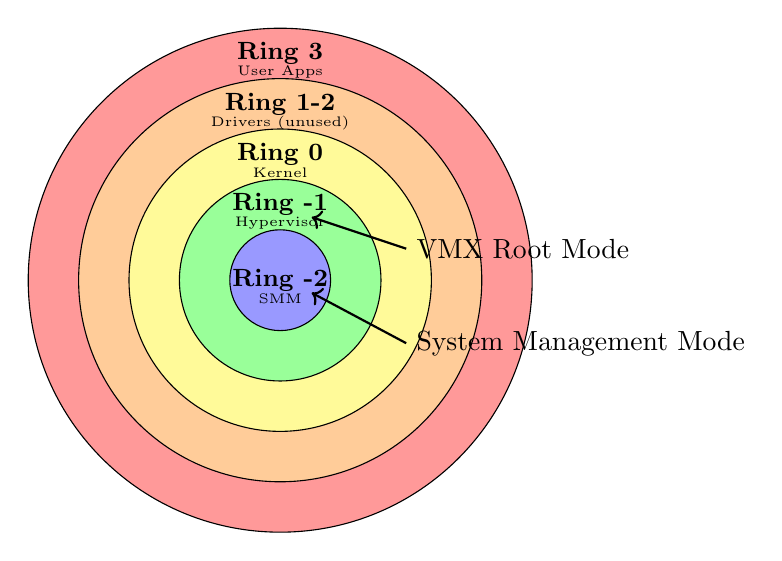
\begin{tikzpicture}[scale=0.8]
            % Draw visible rings first
            \draw[fill=red!40] (0,0) circle (4cm);
            \draw[fill=orange!40] (0,0) circle (3.2cm);
            \draw[fill=yellow!40] (0,0) circle (2.4cm);
            
            % Standard rings labels
            \node at (0,2) {\small \textbf{Ring 0}};
            \node at (0,1.7) {\tiny Kernel};
            
            \node at (0,2.8) {\small \textbf{Ring 1-2}};
            \node at (0,2.5) {\tiny Drivers (unused)};
            
            \node at (0,3.6) {\small \textbf{Ring 3}};
            \node at (0,3.3) {\tiny User Apps};
            
            % Hidden rings revealed on pause
            \onslide<2->{
                \draw[fill=green!40] (0,0) circle (1.6cm);
                \node at (0,1.2) {\small \textbf{Ring -1}};
                \node at (0,0.9) {\tiny Hypervisor};
                \draw[thick,<-] (0.5,1) -- (2,0.5) node[right] {VMX Root Mode};
            }
            
            \onslide<3->{
                \draw[fill=blue!40] (0,0) circle (0.8cm);
                \node at (0,0) {\small \textbf{Ring -2}};
                \node at (0,-0.3) {\tiny SMM};
                \draw[thick,<-] (0.5,-0.2) -- (2,-1) node[right] {System Management Mode};
            }
        \end{tikzpicture}
    \end{center}
    
    \begin{columns}
        \begin{column}{0.5\textwidth}
            \centering
            \textbf{Modern Usage:}
            \begin{itemize}
                \item Only Ring 0 (Kernel) and Ring 3 (User)
                \item Ring 1-2 unused in practice
                \item Ring -1: Hypervisor (VMX root)
                \item Ring -2: SMM firmware
            \end{itemize}
        \end{column}
        \begin{column}{0.5\textwidth}
            \centering
            \textbf{Protection Method:}
            \begin{tcolorbox}[colback=yellow!20]
                Paging-based protection with NX/XD bit
            \end{tcolorbox}
        \end{column}
    \end{columns}
\end{frame}

\begin{frame}{ARM TrustZone - Trusted Execution Environment (TEE)}
    \begin{center}
        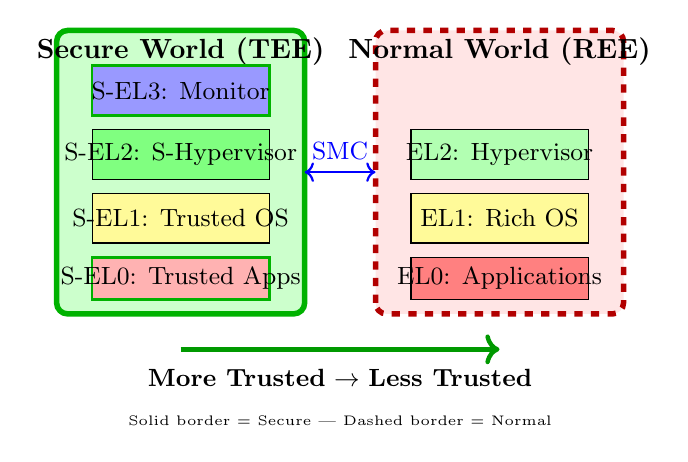
\begin{tikzpicture}[scale=0.9]
            % Secure World - Green gradient with special border
            \draw[fill=green!20,rounded corners,line width=2pt,draw=green!70!black] (-4,0) rectangle (-0.5,4);
            \node at (-2.25,3.7) {\textbf{Secure World (TEE)}};
            
            % Secure levels - gradient from most to least privileged
            \draw[fill=blue!40,draw=green!70!black,line width=1pt] (-3.5,2.8) rectangle (-1,3.5);
            \node at (-2.25,3.15) {\small S-EL3: Monitor};
            
            \draw[fill=green!50] (-3.5,1.9) rectangle (-1,2.6);
            \node at (-2.25,2.25) {\small S-EL2: S-Hypervisor};
            
            \draw[fill=yellow!40] (-3.5,1) rectangle (-1,1.7);
            \node at (-2.25,1.35) {\small S-EL1: Trusted OS};
            
            \draw[fill=red!30,draw=green!70!black,line width=1pt] (-3.5,0.2) rectangle (-1,0.8);
            \node at (-2.25,0.5) {\small S-EL0: Trusted Apps};
            
            % Normal World - Red gradient (untrusted)
            \draw[fill=red!10,rounded corners,line width=2pt,draw=red!70!black,dashed] (0.5,0) rectangle (4,4);
            \node at (2.25,3.7) {\textbf{Normal World (REE)}};
            
            % Normal levels - gradient from kernel to user  
            \draw[fill=green!30] (1,1.9) rectangle (3.5,2.6);
            \node at (2.25,2.25) {\small EL2: Hypervisor};
            
            \draw[fill=yellow!40] (1,1) rectangle (3.5,1.7);
            \node at (2.25,1.35) {\small EL1: Rich OS};
            
            \draw[fill=red!50] (1,0.2) rectangle (3.5,0.8);
            \node at (2.25,0.5) {\small EL0: Applications};
            
            % Trust direction arrow
            \draw[->,ultra thick,green!60!black] (-2.25,-0.5) -- (2.25,-0.5);
            \node at (0,-0.9) {\small \textbf{More Trusted} $\rightarrow$ \textbf{Less Trusted}};
            
            % SMC transition
            \draw[<->,thick,blue] (-0.5,2) -- (0.5,2);
            \node[blue] at (0,2.3) {\small SMC};
            
            % Legend
            \node at (0,-1.5) {\tiny Solid border = Secure | Dashed border = Normal};
        \end{tikzpicture}
    \end{center}
    
    \begin{columns}
        \begin{column}{0.5\textwidth}
            \textbf{TEE Use Cases:}
            \begin{itemize}
                \item DRM content protection
                \item Mobile payments
                \item Biometric authentication
                \item Key management
            \end{itemize}
        \end{column}
        \begin{column}{0.5\textwidth}
            \textbf{TEE = Trusted Execution Environment}
            \begin{itemize}
                \item Isolated from Rich OS (REE)
                \item Secure boot chain
                \item Cryptographic operations
                \item Hardware root of trust
            \end{itemize}
        \end{column}
    \end{columns}
\end{frame}

\begin{frame}{Virtualization Security}
    \begin{columns}
        \begin{column}{0.5\textwidth}
            \textbf{Intel VT-x Features:}
            \begin{itemize}
                \item VMX root/non-root modes
                \item VMCS (VM Control Structure)
                \item EPT (Extended Page Tables)
                \item VPID (Virtual Processor ID)
            \end{itemize}
            
            \vspace{0.3cm}
            \textbf{VM Exits:}
            \begin{itemize}
                \item Privileged instructions
                \item Page faults
                \item I/O operations
                \item MSR access
            \end{itemize}
        \end{column}
        \begin{column}{0.5\textwidth}
            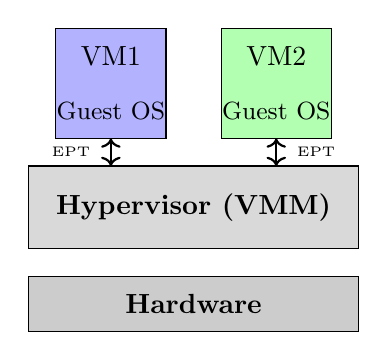
\begin{tikzpicture}[scale=0.7]
                % Hypervisor
                \draw[fill=gray!30] (0,0) rectangle (6,1.5);
                \node at (3,0.75) {\textbf{Hypervisor (VMM)}};
                
                % VMs
                \draw[fill=blue!30] (0.5,2) rectangle (2.5,4);
                \node at (1.5,3.5) {VM1};
                \node at (1.5,2.5) {\small Guest OS};
                
                \draw[fill=green!30] (3.5,2) rectangle (5.5,4);
                \node at (4.5,3.5) {VM2};
                \node at (4.5,2.5) {\small Guest OS};
                
                % EPT arrows
                \draw[<->,thick] (1.5,2) -- (1.5,1.5);
                \node[left] at (1.3,1.75) {\tiny EPT};
                
                \draw[<->,thick] (4.5,2) -- (4.5,1.5);
                \node[right] at (4.7,1.75) {\tiny EPT};
                
                % Hardware
                \draw[fill=black!20] (0,-0.5) rectangle (6,-1.5);
                \node at (3,-1) {\textbf{Hardware}};
            \end{tikzpicture}
        \end{column}
    \end{columns}
\end{frame}

% Management Engines and IOMMU
\begin{frame}{Intel Management Engine (ME)}
    \begin{columns}
        \begin{column}{0.5\textwidth}
            \textbf{What is Intel ME?}
            \begin{itemize}
                \item Separate processor on Intel chipsets
                \item Runs even when main CPU is off
                \item Has full memory/network access
                \item Runs at Ring -3 privilege
                \item Cannot be disabled on modern systems
            \end{itemize}
            
            \vspace{0.3cm}
            \textbf{Legitimate Uses:}
            \begin{itemize}
                \item Remote management (AMT)
                \item DRM enforcement
                \item Boot verification
                \item Anti-theft features
            \end{itemize}
            
            \vspace{0.3cm}
            \textbf{Security Concerns:}
            \begin{itemize}
                \item Closed source firmware
                \item History of vulnerabilities
                \item Potential backdoor vector
            \end{itemize}
        \end{column}
        \begin{column}{0.5\textwidth}
            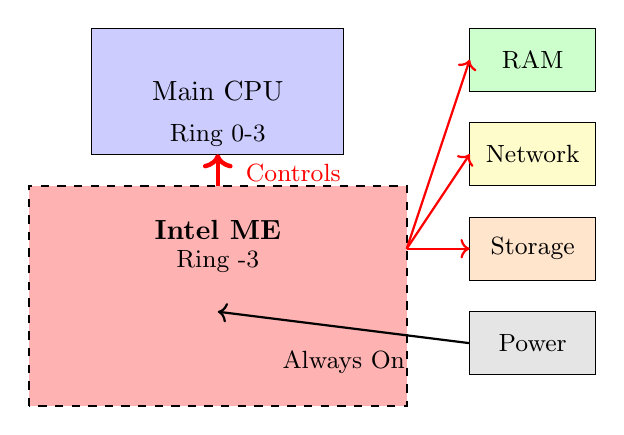
\begin{tikzpicture}[scale=0.8]
                % Main CPU
                \draw[fill=blue!20] (0,4) rectangle (4,6);
                \node at (2,5) {Main CPU};
                \node at (2,4.3) {\small Ring 0-3};
                
                % ME
                \draw[fill=red!30,thick,dashed] (-1,0) rectangle (5,3.5);
                \node at (2,2.8) {\textbf{Intel ME}};
                \node at (2,2.3) {\small Ring -3};
                
                % Resources
                \draw[fill=green!20] (6,5) rectangle (8,6);
                \node at (7,5.5) {\small RAM};
                
                \draw[fill=yellow!20] (6,3.5) rectangle (8,4.5);
                \node at (7,4) {\small Network};
                
                \draw[fill=orange!20] (6,2) rectangle (8,3);
                \node at (7,2.5) {\small Storage};
                
                % ME access arrows
                \draw[->,thick,red] (5,2.5) -- (6,5.5);
                \draw[->,thick,red] (5,2.5) -- (6,4);
                \draw[->,thick,red] (5,2.5) -- (6,2.5);
                
                % ME controls CPU
                \draw[->,ultra thick,red] (2,3.5) -- (2,4);
                \node[red] at (3.2,3.7) {\small Controls};
                
                % Power state
                \draw[fill=gray!20] (6,0.5) rectangle (8,1.5);
                \node at (7,1) {\small Power};
                \draw[->,thick] (6,1) -- (2,1.5);
                \node at (4,0.7) {\small Always On};
            \end{tikzpicture}
            
            \vspace{0.3cm}
            \begin{tcolorbox}[colback=yellow!20]
                \small
                \textbf{Similar Systems:}
                \begin{itemize}
                    \item AMD PSP (Platform Security Processor)
                    \item ARM TrustZone
                \end{itemize}
            \end{tcolorbox}
        \end{column}
    \end{columns}
\end{frame}

\begin{frame}{IOMMU - Input/Output Memory Management Unit}
    \begin{columns}
        \begin{column}{0.5\textwidth}
            \textbf{What is IOMMU?}
            \begin{itemize}
                \item Hardware unit controlling device DMA
                \item Maps device addresses to physical memory
                \item Similar to MMU but for devices
                \item Intel: VT-d, AMD: AMD-Vi
            \end{itemize}
            
            \vspace{0.3cm}
            \textbf{Key Features:}
            \begin{itemize}
                \item \textbf{PASID:} Process Address Space ID
                \begin{itemize}
                    \item Like ASID but for devices
                    \item Allows device access to specific process memory
                \end{itemize}
                \item \textbf{Protection Granularity:} Page-level (4KB)
                \item \textbf{Interrupt Remapping:} Prevents interrupt injection
            \end{itemize}
            
            \vspace{0.3cm}
            \textbf{Attacks Prevented:}
            \begin{itemize}
                \item \textcolor{red}{DMA attacks} (BadUSB, Thunderstrike)
                \item \textcolor{red}{Malicious devices} reading memory
                \item \textcolor{red}{Driver bugs} corrupting memory
            \end{itemize}
        \end{column}
        \begin{column}{0.5\textwidth}
            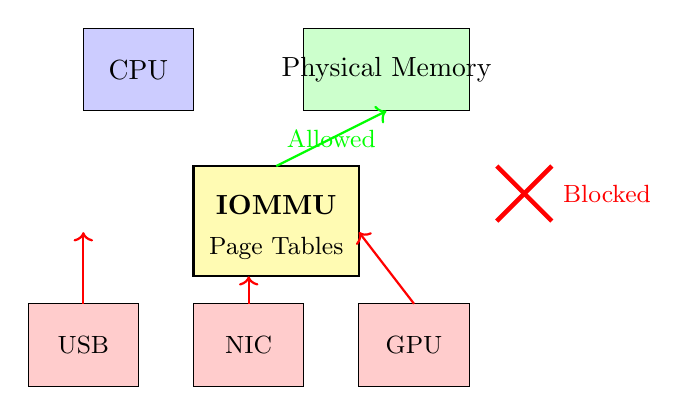
\begin{tikzpicture}[scale=0.7]
                % CPU and Memory
                \draw[fill=blue!20] (0,5) rectangle (2,6.5);
                \node at (1,5.75) {CPU};
                
                \draw[fill=green!20] (4,5) rectangle (7,6.5);
                \node at (5.5,5.75) {Physical Memory};
                
                % IOMMU
                \draw[fill=yellow!30,thick] (2,2) rectangle (5,4);
                \node at (3.5,3.3) {\textbf{IOMMU}};
                \node at (3.5,2.5) {\small Page Tables};
                
                % Devices
                \draw[fill=red!20] (-1,0) rectangle (1,1.5);
                \node at (0,0.75) {\small USB};
                
                \draw[fill=red!20] (2,0) rectangle (4,1.5);
                \node at (3,0.75) {\small NIC};
                
                \draw[fill=red!20] (5,0) rectangle (7,1.5);
                \node at (6,0.75) {\small GPU};
                
                % Device attempts
                \draw[->,thick,red] (0,1.5) -- (0,2.8);
                \draw[->,thick,red] (3,1.5) -- (3,2);
                \draw[->,thick,red] (6,1.5) -- (5,2.8);
                
                % IOMMU filtering
                \draw[->,thick,green] (3.5,4) -- (5.5,5);
                \node[green] at (4.5,4.5) {\small Allowed};
                
                % Blocked access
                \draw[red,ultra thick] (7.5,3) -- (8.5,4);
                \draw[red,ultra thick] (7.5,4) -- (8.5,3);
                \node[red] at (9.5,3.5) {\small Blocked};
            \end{tikzpicture}
            
            \vspace{0.3cm}
            \begin{tcolorbox}[colback=orange!20]
                \small
                \textbf{Rubber Ducky Example:}
                Malicious USB device attempts to read kernel memory via DMA - blocked by IOMMU
            \end{tcolorbox}
            
            \begin{tcolorbox}[colback=yellow!10]
                \small
                \textbf{Challenge:} Buffer sharing requires careful management when protection is page-granular
            \end{tcolorbox}
        \end{column}
    \end{columns}
\end{frame}

\begin{frame}{IOMMU Protection Scenarios}
    \begin{columns}
        \begin{column}{0.5\textwidth}
            \textbf{CPU-Initiated Attacks:}
            \begin{itemize}
                \item Compromised driver attempts DMA
                \item Kernel bug triggers bad DMA request
                \item IOMMU validates all translations
            \end{itemize}
            
            \vspace{0.3cm}
            \textbf{Device-Initiated Attacks:}
            \begin{itemize}
                \item Malicious firmware in peripherals
                \item Compromised network cards
                \item Rogue Thunderbolt devices
                \item USB devices with DMA capability
            \end{itemize}
            
            \vspace{0.3cm}
            \textbf{Shared Buffer Problem:}
            \begin{tcolorbox}[colback=yellow!20]
                \small
                When data structures share a page:
                \begin{itemize}
                    \item Device needs access to buffer A
                    \item Buffer B is on same 4KB page
                    \item Device can access both!
                \end{itemize}
            \end{tcolorbox}
        \end{column}
        \begin{column}{0.5\textwidth}
            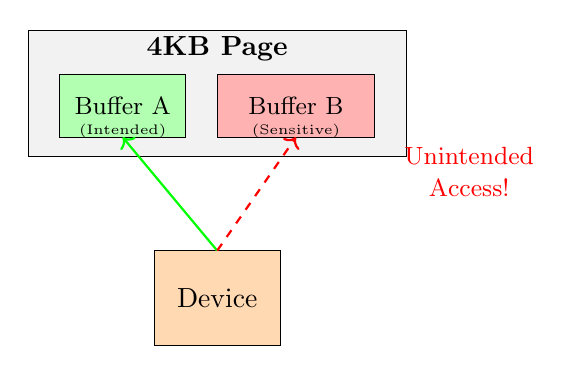
\begin{tikzpicture}[scale=0.8]
                % Memory page
                \draw[fill=gray!10] (0,4) rectangle (6,6);
                \node at (3,5.7) {\textbf{4KB Page}};
                
                % Buffer A
                \draw[fill=green!30] (0.5,4.3) rectangle (2.5,5.3);
                \node at (1.5,4.8) {\small Buffer A};
                \node at (1.5,4.4) {\tiny (Intended)};
                
                % Buffer B
                \draw[fill=red!30] (3,4.3) rectangle (5.5,5.3);
                \node at (4.25,4.8) {\small Buffer B};
                \node at (4.25,4.4) {\tiny (Sensitive)};
                
                % Device
                \draw[fill=orange!30] (2,1) rectangle (4,2.5);
                \node at (3,1.75) {Device};
                
                % Access arrows
                \draw[->,thick,green] (3,2.5) -- (1.5,4.3);
                \draw[->,thick,red,dashed] (3,2.5) -- (4.25,4.3);
                
                \node[red] at (7,4) {\small Unintended};
                \node[red] at (7,3.5) {\small Access!};
            \end{tikzpicture}
            
            \vspace{0.3cm}
            \begin{tcolorbox}[colback=blue!20]
                \small
                \textbf{Solutions:}
                \begin{itemize}
                    \item Align DMA buffers to page boundaries
                    \item Use bounce buffers
                    \item Sub-page protection (future)
                \end{itemize}
            \end{tcolorbox}
        \end{column}
    \end{columns}
\end{frame}

% Section 4: Trusted Execution
\section{Trusted Execution Environments}

\begin{frame}{Intel TDX (Trust Domain Extensions)}
    \begin{columns}
        \begin{column}{0.5\textwidth}
            \textbf{Who Protects Whom:}
            \begin{itemize}
                \item \textcolor{green!70!black}{\textbf{Protected:}} Guest VMs
                \item \textcolor{red}{\textbf{Threat:}} Cloud Provider
                \item \textcolor{blue}{\textbf{Enforcer:}} CPU Hardware
            \end{itemize}
            
            \vspace{0.3cm}
            \textbf{Protection Guarantees:}
            \begin{itemize}
                \item Confidentiality from hypervisor
                \item Memory encryption per VM
                \item CPU-attested execution
                \item Secure EPT (S-EPT)
            \end{itemize}
            
            \vspace{0.3cm}
            \textbf{Use Case:}
            \begin{tcolorbox}[colback=green!10]
                \small
                Run sensitive workloads on untrusted cloud infrastructure
            \end{tcolorbox}
        \end{column}
        \begin{column}{0.5\textwidth}
            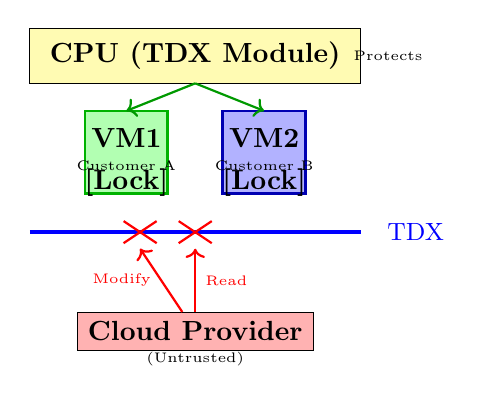
\begin{tikzpicture}[scale=0.7]
                % Threat Actor
                \node[draw,fill=red!30,minimum width=3cm] (provider) at (0,0) {\textbf{Cloud Provider}};
                \node at (0,-0.5) {\tiny (Untrusted)};
                
                % Attack attempts
                \draw[->,thick,red] (provider) -- (0,1.5) node[midway,right] {\tiny Read};
                \draw[->,thick,red] (provider) -- (-1,1.5) node[midway,left] {\tiny Modify};
                
                % Protection barrier
                \draw[ultra thick,blue] (-3,1.8) -- (3,1.8);
                \node[blue] at (4,1.8) {\small TDX};
                \draw[thick,red] (-0.3,1.6) -- (0.3,2);
                \draw[thick,red] (0.3,1.6) -- (-0.3,2);
                \draw[thick,red] (-1.3,1.6) -- (-0.7,2);
                \draw[thick,red] (-0.7,1.6) -- (-1.3,2);
                
                % Protected VMs
                \draw[fill=green!30,draw=green!70!black,line width=1pt] (-2,2.5) rectangle (-0.5,4);
                \node at (-1.25,3.5) {\textbf{VM1}};
                \node at (-1.25,3) {\tiny Customer A};
                \node at (-1.25,2.7) {\textbf{[Lock]}};
                
                \draw[fill=blue!30,draw=blue!70!black,line width=1pt] (0.5,2.5) rectangle (2,4);
                \node at (1.25,3.5) {\textbf{VM2}};
                \node at (1.25,3) {\tiny Customer B};
                \node at (1.25,2.7) {\textbf{[Lock]}};
                
                % CPU enforcement
                \draw[fill=yellow!30] (-3,4.5) rectangle (3,5.5);
                \node at (0,5) {\textbf{CPU (TDX Module)}};
                
                % Protection arrows
                \draw[->,thick,green!60!black] (0,4.5) -- (-1.25,4);
                \draw[->,thick,green!60!black] (0,4.5) -- (1.25,4);
                \node at (3.5,5) {\tiny Protects};
            \end{tikzpicture}
        \end{column}
    \end{columns}
\end{frame}

\begin{frame}{Intel SGX Enclaves}
    \begin{columns}
        \begin{column}{0.5\textwidth}
            \textbf{SGX - Another TEE Implementation:}
            \begin{itemize}
                \item Isolated execution environment (TEE)
                \item Encrypted memory (MEE)
                \item Remote attestation
                \item Sealed storage
                \item x86-specific (vs ARM TrustZone)
            \end{itemize}
            
            \vspace{0.3cm}
            \textbf{Instructions:}
            \begin{itemize}
                \item \texttt{ECREATE}: Create enclave
                \item \texttt{EENTER}: Enter enclave
                \item \texttt{EEXIT}: Exit enclave
                \item \texttt{ERESUME}: Resume after AEX
            \end{itemize}
        \end{column}
        \begin{column}{0.5\textwidth}
            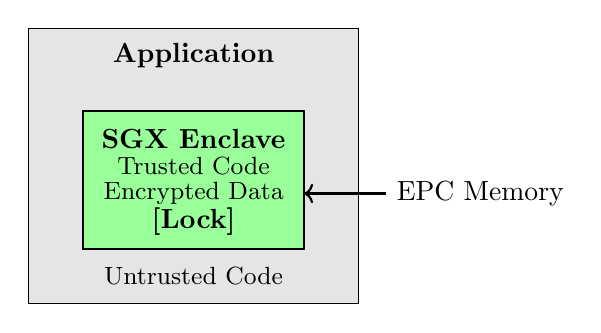
\begin{tikzpicture}[scale=0.7]
                % Application
                \draw[fill=gray!20] (0,0) rectangle (6,5);
                \node at (3,4.5) {\textbf{Application}};
                
                % Enclave
                \draw[fill=green!40,thick] (1,1) rectangle (5,3.5);
                \node at (3,3) {\textbf{SGX Enclave}};
                \node at (3,2.5) {\small Trusted Code};
                \node at (3,2) {\small Encrypted Data};
                \node at (3,1.5) {\textbf{[Lock]}};
                
                % Untrusted part
                \node at (3,0.5) {\small Untrusted Code};
                
                % EPC
                \draw[<-,thick] (5,2) -- (6.5,2) node[right] {EPC Memory};
            \end{tikzpicture}
            
            \vspace{0.3cm}
            \textbf{Page Types:}
            REG, TCS, SECS, VA
        \end{column}
    \end{columns}
\end{frame}

\begin{frame}{MKTME (Multi-Key Total Memory Encryption)}
    \begin{columns}
        \begin{column}{0.5\textwidth}
            \textbf{Features:}
            \begin{itemize}
                \item Multiple encryption keys
                \item Per-VM/container isolation
                \item KeyID in physical address bits
                \item AES-XTS encryption
            \end{itemize}
            
            \vspace{0.3cm}
            \textbf{Key Management:}
            \begin{itemize}
                \item Up to 15 keys (4-bit KeyID)
                \item Software-managed keys
                \item PCONFIG instruction
                \item Key rotation support
            \end{itemize}
        \end{column}
        \begin{column}{0.5\textwidth}
            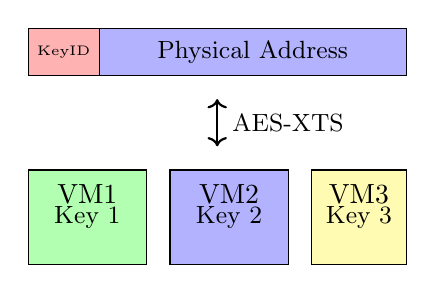
\begin{tikzpicture}[scale=0.6]
                % Physical address
                \draw (0,4) rectangle (8,5);
                \draw[fill=red!30] (0,4) rectangle (1.5,5);
                \draw[fill=blue!30] (1.5,4) rectangle (8,5);
                \node at (0.75,4.5) {\tiny KeyID};
                \node at (4.75,4.5) {\small Physical Address};
                
                % Memory regions
                \draw[fill=green!30] (0,0) rectangle (2.5,2);
                \node at (1.25,1.5) {VM1};
                \node at (1.25,1) {\small Key 1};
                
                \draw[fill=blue!30] (3,0) rectangle (5.5,2);
                \node at (4.25,1.5) {VM2};
                \node at (4.25,1) {\small Key 2};
                
                \draw[fill=yellow!30] (6,0) rectangle (8,2);
                \node at (7,1.5) {VM3};
                \node at (7,1) {\small Key 3};
                
                % Encryption engine
                \draw[thick,<->] (4,2.5) -- (4,3.5);
                \node at (5.5,3) {\small AES-XTS};
            \end{tikzpicture}
            
            \vspace{0.3cm}
            \textbf{Use Cases:}
            \begin{itemize}
                \item Cloud multi-tenancy
                \item Container isolation
                \item Key-based memory domains
            \end{itemize}
        \end{column}
    \end{columns}
\end{frame}

% Section 5: Boot Security
\section{Boot Security}

\begin{frame}{Secure Boot}
    \begin{columns}
        \begin{column}{0.5\textwidth}
            \textbf{UEFI Secure Boot Chain:}
            \begin{enumerate}
                \item Platform Key (PK)
                \item Key Exchange Keys (KEK)
                \item Signature Database (db)
                \item Forbidden Signatures (dbx)
            \end{enumerate}
            
            \vspace{0.3cm}
            \textbf{Boot Stages:}
            \begin{itemize}
                \item SEC: Security phase
                \item PEI: Pre-EFI Init
                \item DXE: Driver Execution
                \item BDS: Boot Device Select
                \item OS Loader verification
            \end{itemize}
        \end{column}
        \begin{column}{0.5\textwidth}
            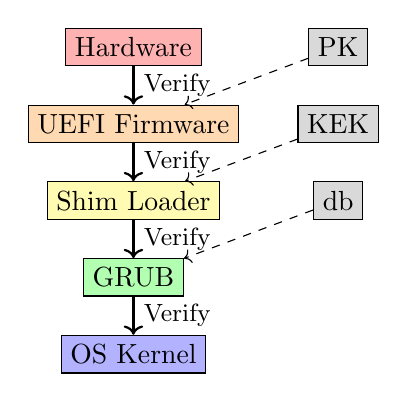
\begin{tikzpicture}[scale=0.65]
                % Boot chain
                \node[draw,fill=red!30] (hw) at (0,0) {Hardware};
                \node[draw,fill=orange!30] (uefi) at (0,-1.5) {UEFI Firmware};
                \node[draw,fill=yellow!30] (shim) at (0,-3) {Shim Loader};
                \node[draw,fill=green!30] (grub) at (0,-4.5) {GRUB};
                \node[draw,fill=blue!30] (kernel) at (0,-6) {OS Kernel};
                
                % Verification arrows
                \draw[->,thick] (hw) -- (uefi) node[midway,right] {\small Verify};
                \draw[->,thick] (uefi) -- (shim) node[midway,right] {\small Verify};
                \draw[->,thick] (shim) -- (grub) node[midway,right] {\small Verify};
                \draw[->,thick] (grub) -- (kernel) node[midway,right] {\small Verify};
                
                % Keys
                \node[draw,fill=gray!30] (pk) at (4,0) {PK};
                \node[draw,fill=gray!30] (kek) at (4,-1.5) {KEK};
                \node[draw,fill=gray!30] (db) at (4,-3) {db};
                
                % Key relationships
                \draw[dashed,->] (pk) -- (uefi);
                \draw[dashed,->] (kek) -- (shim);
                \draw[dashed,->] (db) -- (grub);
            \end{tikzpicture}
        \end{column}
    \end{columns}
\end{frame}

\begin{frame}{Chain of Trust and UEFI Vulnerabilities}
    \begin{columns}
        \begin{column}{0.5\textwidth}
            \textbf{Chain of Trust Concept:}
            \begin{itemize}
                \item Each component verifies the next
                \item Trust anchored in hardware
                \item Weakest link breaks entire chain
            \end{itemize}
            
            \vspace{0.3cm}
            \textbf{UEFI as Attack Surface:}
            \begin{itemize}
                \item \textcolor{red}{Complex codebase (millions of LOC)}
                \item \textcolor{red}{Third-party drivers/modules}
                \item \textcolor{red}{Network stack in firmware}
                \item \textcolor{red}{Persistent across OS reinstalls}
            \end{itemize}
            
            \vspace{0.3cm}
            \textbf{Known UEFI Attacks:}
            \begin{itemize}
                \item BootHole (CVE-2020-10713)
                \item LogoFAIL (2023)
                \item BlackLotus bootkit
                \item ThinkPwn vulnerabilities
            \end{itemize}
        \end{column}
        \begin{column}{0.5\textwidth}
            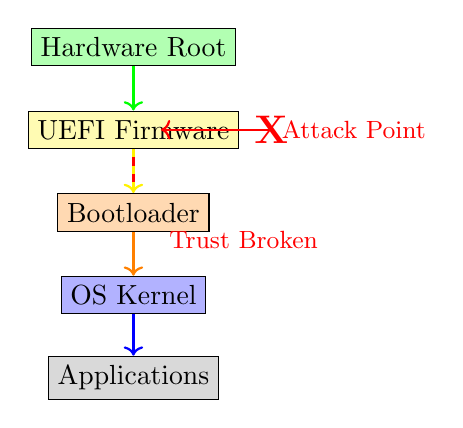
\begin{tikzpicture}[scale=0.7]
                % Chain links
                \node[draw,fill=green!30] (hw) at (0,0) {Hardware Root};
                \node[draw,fill=yellow!30] (uefi) at (0,-1.5) {UEFI Firmware};
                \node[draw,fill=orange!30] (boot) at (0,-3) {Bootloader};
                \node[draw,fill=blue!30] (os) at (0,-4.5) {OS Kernel};
                \node[draw,fill=gray!30] (app) at (0,-6) {Applications};
                
                % Trust flow
                \draw[->,thick,green] (hw) -- (uefi);
                \draw[->,thick,yellow] (uefi) -- (boot);
                \draw[->,thick,orange] (boot) -- (os);
                \draw[->,thick,blue] (os) -- (app);
                
                % Attack point
                \node[red,thick] at (2.5,-1.5) {\Large \textbf{X}};
                \draw[->,red,thick] (2.5,-1.5) -- (0.5,-1.5);
                \node[red] at (4,-1.5) {\small Attack Point};
                
                % Broken chain
                \draw[red,thick,dashed] (0,-2) -- (0,-2.5);
                \node[red] at (2,-3.5) {\small Trust Broken};
            \end{tikzpicture}
            
            \vspace{0.3cm}
            \begin{tcolorbox}[colback=red!10]
                \textbf{Critical Issue:}
                UEFI compromise gives attacker:
                \begin{itemize}
                    \item Ring -2 privileges
                    \item Persistence below OS
                    \item Bypass of all OS security
                \end{itemize}
            \end{tcolorbox}
        \end{column}
    \end{columns}
\end{frame}

\begin{frame}{TPM - Trusted Platform Module}
    \begin{columns}
        \begin{column}{0.5\textwidth}
            \textbf{What is TPM?}
            \begin{itemize}
                \item Hardware security chip
                \item Cryptographic processor
                \item Tamper-resistant storage
                \item Platform integrity measurement
            \end{itemize}
            
            \vspace{0.3cm}
            \textbf{TPM Capabilities:}
            \begin{itemize}
                \item Random number generation
                \item Secure key generation/storage
                \item Platform attestation
                \item Sealed storage (bind to PCR state)
            \end{itemize}
            
            \vspace{0.3cm}
            \textbf{TPM Versions:}
            \begin{itemize}
                \item TPM 1.2: SHA-1, RSA
                \item TPM 2.0: SHA-256, ECC support
            \end{itemize}
        \end{column}
        \begin{column}{0.5\textwidth}
            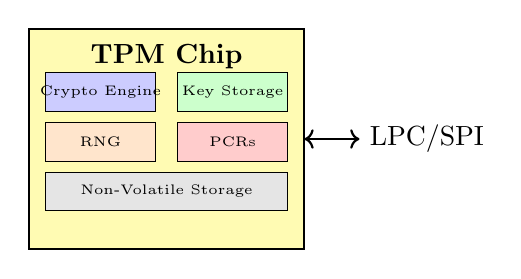
\begin{tikzpicture}[scale=0.7]
                % TPM Chip
                \draw[fill=yellow!30,thick] (0,0) rectangle (5,4);
                \node at (2.5,3.5) {\textbf{TPM Chip}};
                
                % Components
                \draw[fill=blue!20] (0.3,2.5) rectangle (2.3,3.2);
                \node at (1.3,2.85) {\tiny Crypto Engine};
                
                \draw[fill=green!20] (2.7,2.5) rectangle (4.7,3.2);
                \node at (3.7,2.85) {\tiny Key Storage};
                
                \draw[fill=orange!20] (0.3,1.6) rectangle (2.3,2.3);
                \node at (1.3,1.95) {\tiny RNG};
                
                \draw[fill=red!20] (2.7,1.6) rectangle (4.7,2.3);
                \node at (3.7,1.95) {\tiny PCRs};
                
                \draw[fill=gray!20] (0.3,0.7) rectangle (4.7,1.4);
                \node at (2.5,1.05) {\tiny Non-Volatile Storage};
                
                % External connections
                \draw[<->,thick] (5,2) -- (6,2) node[right] {LPC/SPI};
            \end{tikzpicture}
            
            \vspace{0.3cm}
            \textbf{Use Cases:}
            \begin{itemize}
                \item BitLocker/LUKS disk encryption
                \item Measured/Secure Boot
                \item Remote attestation
                \item VPN client certificates
            \end{itemize}
        \end{column}
    \end{columns}
\end{frame}

\begin{frame}{Measured Boot with TPM}
    \begin{columns}
        \begin{column}{0.5\textwidth}
            \textbf{Platform Configuration Registers:}
            \begin{itemize}
                \item PCR0-7: BIOS/UEFI measurements
                \item PCR8-9: OS Loader configuration
                \item PCR10: IMA (Linux integrity)
                \item PCR11-15: OS-specific
                \item PCR16-23: Debug/Vendor-specific
            \end{itemize}
            
            \vspace{0.3cm}
            \textbf{PCR Extend Operation:}
            \begin{tcolorbox}[colback=gray!10]
                \small
                PCR[i] = SHA256(PCR[i] || data)
            \end{tcolorbox}
            \small Cannot directly write PCRs!
        \end{column}
        \begin{column}{0.5\textwidth}
            \textbf{Boot Measurement Chain:}
            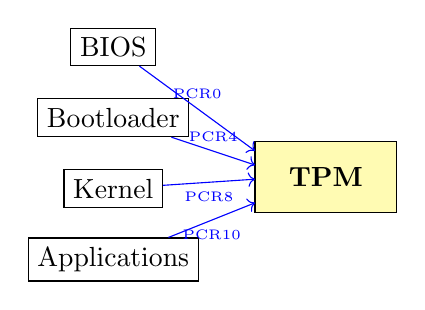
\begin{tikzpicture}[scale=0.6]
                % Components
                \node[draw] (bios) at (0,0) {BIOS};
                \node[draw] (mbr) at (0,-1.5) {Bootloader};
                \node[draw] (kernel) at (0,-3) {Kernel};
                \node[draw] (apps) at (0,-4.5) {Applications};
                
                % TPM
                \draw[fill=yellow!30] (3,-2) rectangle (6,-3.5);
                \node at (4.5,-2.75) {\textbf{TPM}};
                
                % Measurements
                \draw[->,blue] (bios) -- (3,-2.2) node[midway,above] {\tiny PCR0};
                \draw[->,blue] (mbr) -- (3,-2.5) node[midway,above] {\tiny PCR4};
                \draw[->,blue] (kernel) -- (3,-2.8) node[midway,below] {\tiny PCR8};
                \draw[->,blue] (apps) -- (3,-3.3) node[midway,below] {\tiny PCR10};
            \end{tikzpicture}
            
            \vspace{0.3cm}
            \textbf{Attestation:}
            \begin{itemize}
                \item Quote = Sign(PCRs, AIK)
                \item Proves system state to remote party
                \item Unsealing secrets based on PCR values
            \end{itemize}
        \end{column}
    \end{columns}
\end{frame}

% Section 6: Summary
\section{Summary}

\begin{frame}{Hardware Security Evolution}
    \begin{center}
        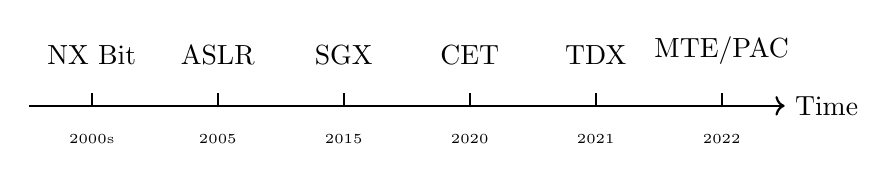
\begin{tikzpicture}[scale=0.8]
            % Timeline
            \draw[thick,->] (0,0) -- (12,0) node[right] {Time};
            
            % Security features
            \node[above] at (1,0.5) {NX Bit};
            \draw[thick] (1,0) -- (1,0.2);
            \node[below] at (1,-0.3) {\tiny 2000s};
            
            \node[above] at (3,0.5) {ASLR};
            \draw[thick] (3,0) -- (3,0.2);
            \node[below] at (3,-0.3) {\tiny 2005};
            
            \node[above] at (5,0.5) {SGX};
            \draw[thick] (5,0) -- (5,0.2);
            \node[below] at (5,-0.3) {\tiny 2015};
            
            \node[above] at (7,0.5) {CET};
            \draw[thick] (7,0) -- (7,0.2);
            \node[below] at (7,-0.3) {\tiny 2020};
            
            \node[above] at (9,0.5) {TDX};
            \draw[thick] (9,0) -- (9,0.2);
            \node[below] at (9,-0.3) {\tiny 2021};
            
            \node[above] at (11,0.5) {MTE/PAC};
            \draw[thick] (11,0) -- (11,0.2);
            \node[below] at (11,-0.3) {\tiny 2022};
        \end{tikzpicture}
    \end{center}
    
    \vspace{0.5cm}
    \begin{columns}
        \begin{column}{0.5\textwidth}
            \textbf{Current Trends:}
            \begin{itemize}
                \item Hardware-software co-design
                \item Confidential computing
                \item Memory safety focus
                \item Supply chain security
            \end{itemize}
        \end{column}
        \begin{column}{0.5\textwidth}
            \textbf{Challenges:}
            \begin{itemize}
                \item Performance overhead
                \item Compatibility issues
                \item Side-channel attacks
                \item Ecosystem adoption
            \end{itemize}
        \end{column}
    \end{columns}
\end{frame}

\begin{frame}{Key Takeaways}
    \begin{itemize}
        \item \textbf{Defense in Depth:} Multiple layers of security mechanisms
        \vspace{0.3cm}
        \item \textbf{Hardware Acceleration:} Critical security features need hardware support for performance
        \vspace{0.3cm}
        \item \textbf{Trust Boundaries:} Clear separation between trusted and untrusted components
        \vspace{0.3cm}
        \item \textbf{Attestation:} Cryptographic proof of system state and configuration
        \vspace{0.3cm}
        \item \textbf{Memory Protection:} Tags, authentication, and encryption for memory safety
        \vspace{0.3cm}
        \item \textbf{Control Flow:} Hardware enforcement of valid program execution paths
    \end{itemize}
    
    \vspace{0.5cm}
    \begin{tcolorbox}[colback=blue!20]
        \centering
        \textbf{Future:} Homomorphic encryption, quantum-resistant crypto, AI-driven security
    \end{tcolorbox}
\end{frame}

\begin{frame}
    \begin{center}
    {\Huge Questions?}
    
    \vspace{1cm}
    {\Large Thank You!}
    \end{center}
\end{frame}

\end{document}